% !TeX root = ../main.tex
% Add the above to each chapter to make compiling the PDF easier in some editors.

\chapter{Häufigkeiten der Feintypen}\label{chapter:Haeufigkeit_Feintypen}
Abbildung \ref{fig:Eintrittswahrscheinlichkeit} stellt die Risiko-Kategorien und Unterteilung der Eintrittswahrscheinlichkeit, der Feintypen, in vier Bereichen dar. Die Risiko-Kategorien wurden mit verschiedenen Farben markiert, dies vereinfacht die Zuordnung der Feintypen.

\begin{savenotes}
	\begin{figure}[H]
		\centering
		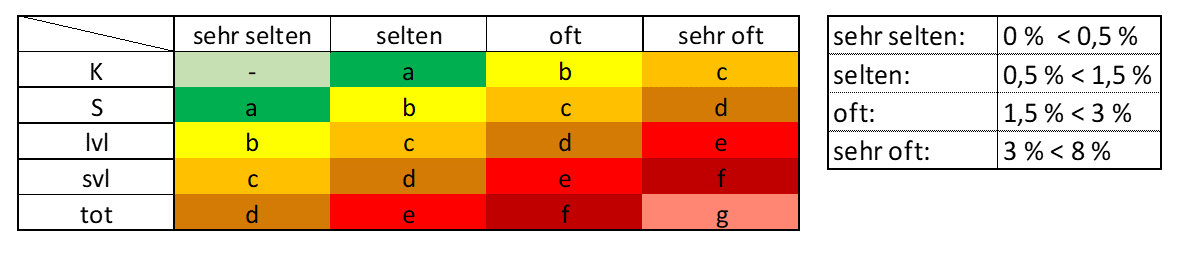
\includegraphics[width=16cm,height=4cm]{figures/Eintrittswahrscheinlichkeit}
		\caption[Bestimmung der Risiko-Kategorie anhand der Eintrittswahrscheinlichkeit und Unfallschwere]{Bestimmung der Risiko Kategorie anhand der Eintrittswahrscheinlichkeit und Unfallschwere}\label{fig:Eintrittswahrscheinlichkeit}
	\end{figure}
\end{savenotes}

Die folgende Tabelle stellt die berechneten Häufigkeiten der einzelnen Feintypen, je nach Schweregrad, dar. Die Häufigkeit wurde nach dem Vorgehen in Kapitel \ref{subsection:Bewertungsskala} bestimmt. Damit die Risiko-Kategorie direkt abgelesen werden kann, wurden die Bereiche farblich markiert. Die höchste Risiko-Kategorie, welche innerhalb eines Feintyps auftritt, ist maßgebend. Die Feintypen selbst wurden mit der Farbe der maßgebenden Kategorie markiert. Die hier berechneten Häufigkeiten werden in den Diagrammen in Kapitel \ref{subsection:Bewertung der typisierten Unfälle} verwendet.
  
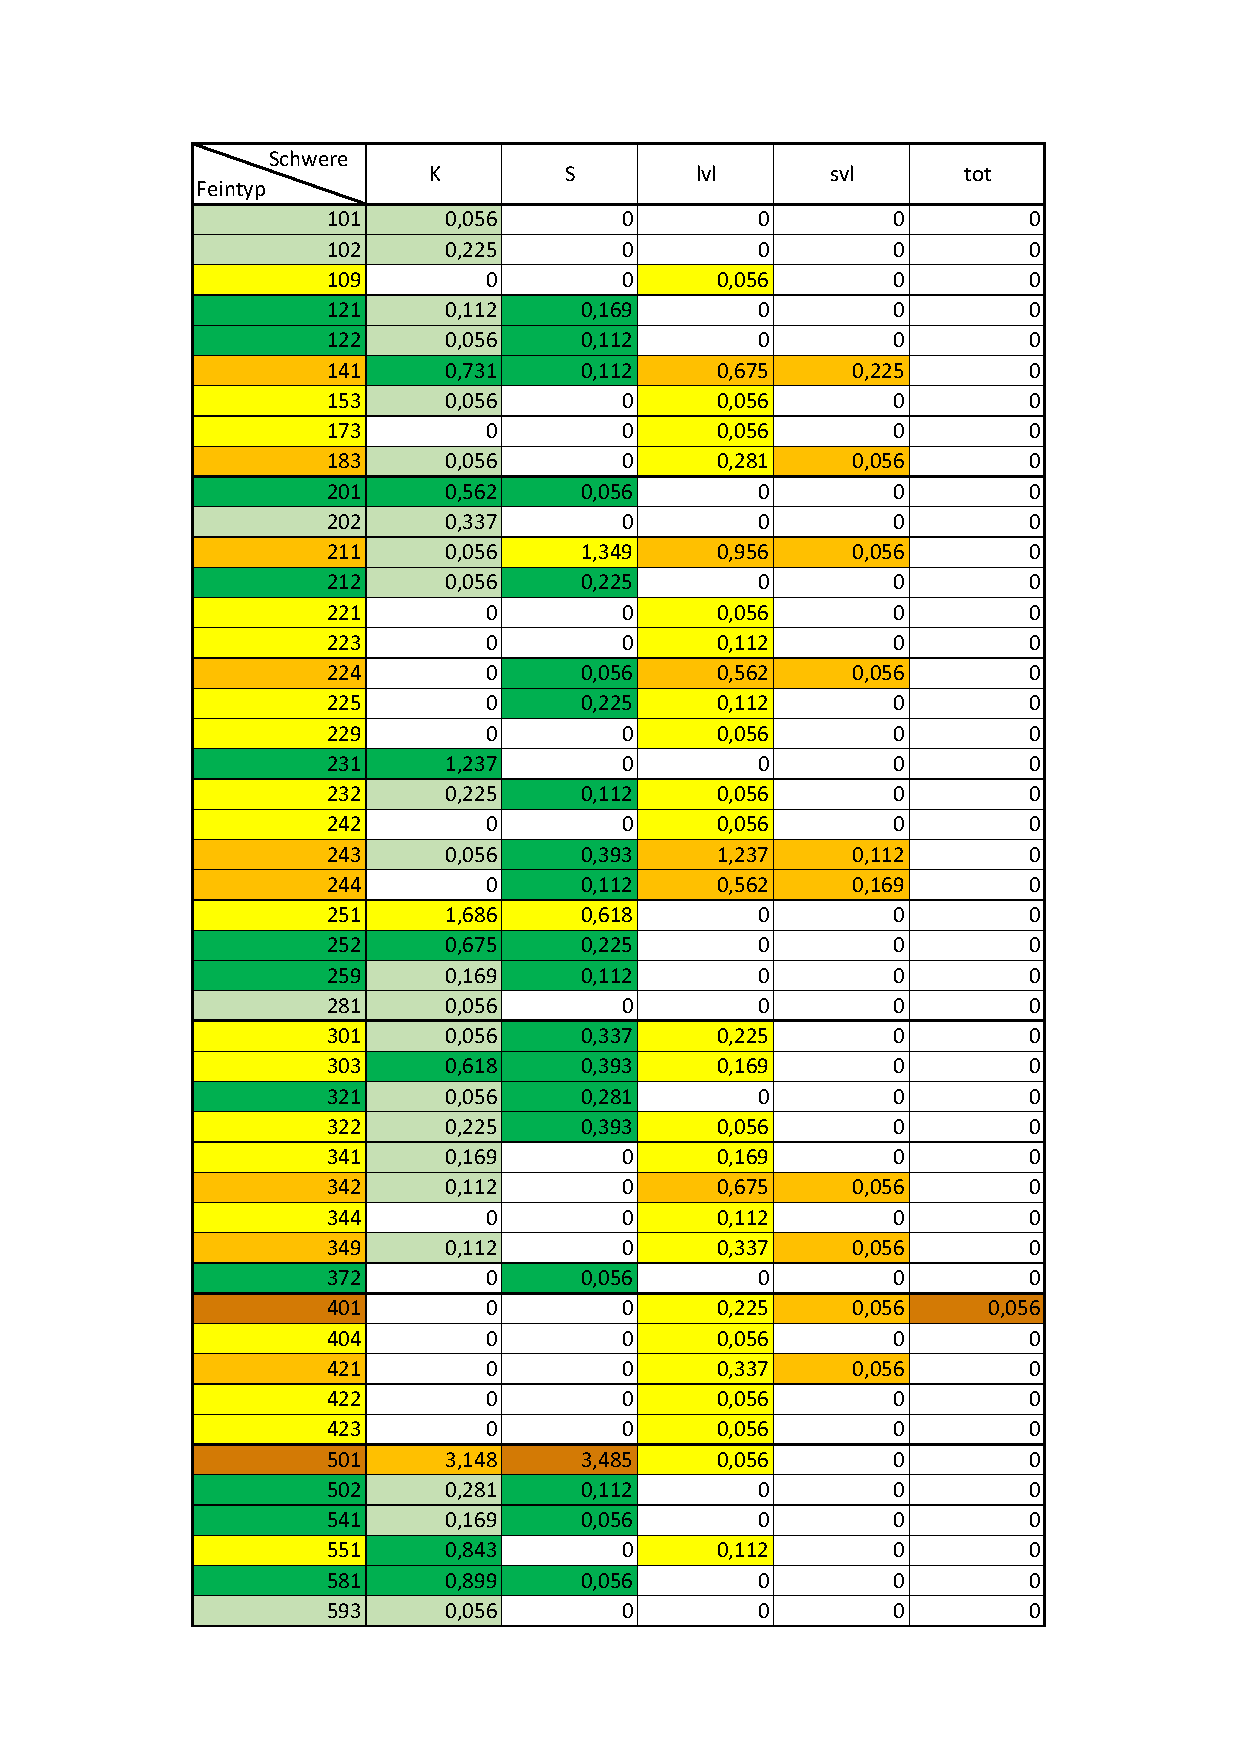
\includepdf[pages={1-2}, pagecommand={\thispagestyle{fancy}}, width=\textwidth, height=\textheight, frame=false]{figures/Feintypen.pdf}
